\chapter{Cinemática de fluidos}
\section{Descripción Euleriana y Lagrangiana}
	
	Dos formas de identificación de las magnitudes (p. e., la velocidad) 
	\begin{enumerate}
		\item {\textbf{\textcolor{red}{Euleriana}}: \\
			Segun la \textcolor{blue}{posición} y el instante. 
		\begin{equation}
			\vec{u}(\vec{x},t)
		\end{equation}
		} 
		\item {\textbf{\textcolor{red}{Lagrangiana}}:\\
			Según la \textcolor{blue}{partí cula} y el instante. La partí cula
			queda identificada (marcada) mediante un vector $\vec{a}$ que puede
			ser, por ejemplo, la posición que tiene la partí cula en un instante
			de referencia $t_{0}$ 
			
\begin{equation}
				\vec{u}(\vec{a},t;t_{0})
\end{equation}
			
		} 
	\end{enumerate}


\section{Lineas de corriente, trayectorias y lineas de traza}

	
	\begin{itemize}
		\item \textcolor{red}{Lineas de corriente}:\\
		Para un instante dado $t_0$, és la tangente a los vectores de velocidad. 
	\end{itemize}

\begin{center}
	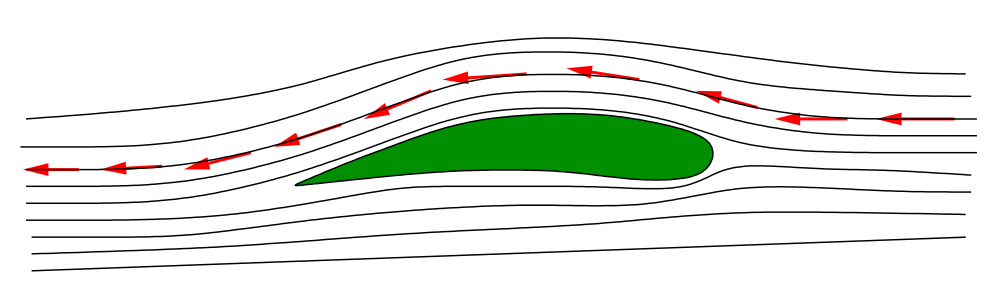
\includegraphics[width=0.7\linewidth]{TeX_files/chapter03-Cinematica/lineasCorriente}
\end{center}

		
		Són solución de la ecuación (en 2D) 
		
		\begin{equation}
			\frac{\text{d}x}{u(\vec{x},t=t_0)}=\frac{\text{d}y}{v(\vec{x},t=t_0)}
		\end{equation}
		


	
	\begin{itemize}
		\item \textcolor{red}{Trayectoria}:\\
		Para una cierta partícula de fluido, puntos que ocupa en un cierto
		intervalo de tiempo. 
		\item \textcolor{red}{Lineas de traza}:\\
		Partículas de fluido que, en un cierto instante anterior, pasaron
		por un determinado punto.
	\end{itemize}
\begin{center}
	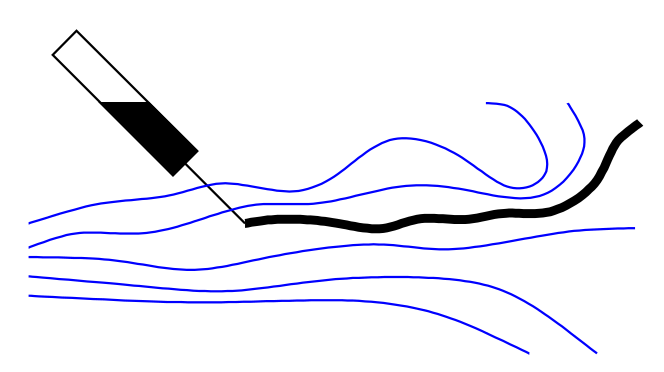
\includegraphics[width=0.5\linewidth]{TeX_files/chapter03-Cinematica/traza}
\end{center}


		
		Si el flujo es estacionario (no depende del tiempo), linea de corriente,
		trayectoria y linea de traza coinciden para un determinado punto. 
		



	
\subsection*{Actividad 1:}
		Dado el campo de velocidades bidimensional $\vec{u}=(x+t)\vec{\imath}+y\vec{\jmath}$,
		encontrad las expresiones para:
		
		a) la linea de corriente que pasa por $(1,1)$ para $t=0$
		
		b) la trayectoria de la partícula que está en $(1,1)$ para $t=0$
		
		c) la línea de traza, para $t=0$, de todas las partículas que pasaron
		por $(1,1)$


\section{Derivada sustancial}

	
	La partícula $P$, en el instante $t$ se encuentra en $\vec{x}$
	con una velocidad $\vec{u}$. La aceleración de $P$ \textbf{no} és
	$\dparc{\vec{u}}{t}$, ya que aunque $\vec{u}$ sea estacionario,
	$P$ puede estar moviéndose a un punto en que $\vec{u}$ és diferente.
	
	En un instante $t+\delta t$, $P$ estará en $\vec{x}+\delta\vec{x}=\vec{x}+\vec{u}\delta t$,
	de forma que la variación de velocidad será 
	\[
	\delta\vec{u}=\vec{u}(\vec{x}+\vec{u}\delta t,t+\delta t)-\vec{u}(\vec{x},t)
	\]
	
	Desarrollando en serie de Taylor hasta primer orden, obtenemos 
	\[
	\delta\vec{u}=\dparc{\vec{u}}{t}\delta t+(\vec{u}\cdot\vec{\nabla})\vec{u}\delta t+O(\delta t^{2}),
	\]
	de forma que la aceleración és 
	\[
	\vec{a}(\vec{x},t)=\dparc{\vec{u}}{t}+(\vec{u}\cdot\vec{\nabla})\vec{u}
	\]
	

De forma general, consideremos cualquier magnitud $f$, asociada a
una propiedad del fluido (puede ser un escalar como la temperatura,
o densidad, o la velocidad angular). 
\begin{itemize}
	\item Derivada \textcolor{red}{local}: 
	\[
	\dparc{f}{t}
	\]
	
	\item Derivada \textcolor{red}{convectiva}: 
	\[
	(\vec{u}\cdot\vec{\nabla})\vec{f}=\left(u\dparc{\phantom{f}}{x}+v\dparc{\phantom{f}}{y}+w\dparc{\phantom{f}}{z}\right)f=u_{i}\dparc{f}{x_{i}}
	\]
	
	\item Derivada \textcolor{red}{sustancial} o \textcolor{red}{total}: 
	\[
	\frac{\text{D}f}{\text{D}t}=\dparc{f}{t}+(\vec{u}\cdot\vec{\nabla})\vec{f}=\dparc{f}{t}+u_{i}\dparc{f}{x_{i}}
	\]
	
\end{itemize}

\section{Circulación, Flujo y Vorticidad}

	
	\begin{itemize}
		\item \textbf{\textcolor{red}{Circulación}}\\
		
		\[
		\Gamma=\oint_{L}\vec{u}\cdot\text{d}\vec{l}
		\]
		$L$ es cualquier contorno cerrado.
	\end{itemize}
	Si este contorno está constituido siempre por las mismas partí culas
	(es decir, es una línea material), se puede demostrar (\cite{Virto1})
	que 
	\[
	\Deriv{\Gamma}{t}=\Deriv{\phantom{t}}{t}\oint_{L}\vec{u}\cdot\text{d}\vec{l}=0
	\]
	

	
	\begin{itemize}
		\item \textbf{\textcolor{red}{Flujo}}\\
		Sea $F$ una magnitud extensiva propiedad del fluido y $f$ esta
		misma magnitud por unidad de volumen. El flujo de $f$ a través de
		la superficie $S$ es
	\end{itemize}
	\[
	\Phi=\int_{S}f\vec{u}\cdot\text{d}\vec{S}
	\]
	Si $f$ es un escalar, $f\vec{u}$ es el \textcolor{blue}{vector
		flujo} de $f$.
	
	Si $f$ es un vector $\left(\vec{f}\right)$ , $\vec{f}\vec{u}$ es
	el \textcolor{blue}{tensor flujo} de $f$.

	
{Ejemplo:}
		
		\[
		f=1\rightarrow\begin{cases}
			\vec{u} & \textrm{vector flujo volumétrico}\\
			Q=\int_{S}\vec{u}\cdot\text{d}\vec{S} & \textrm{flujo volumétrico, o caudal}
		\end{cases}
		\]
		
		\[
		f=\rho\rightarrow\begin{cases}
			\rho\vec{u} & \textrm{vector flujo másico}\\
			\dot{m}=\int_{S}\rho\vec{u}\cdot\text{d}\vec{S} & \textrm{flujo másico, o gasto}
		\end{cases}
		\]
		

\begin{itemize}
	\item \textbf{\textcolor{red}{Vorticidad}}\\
	
	\[
	\vec{\omega}=\vec{\nabla}\times\vec{u}\quad\text{En componentes:}\quad\omega_{k}=-\varepsilon_{ijk}\dparc{u_{i}}{x_{j}}
	\]
	Es el doble de la velocidad local de rotación del elemento de fluido.
	Por definición de vorticidad, se cumple que 
	\[
	\vec{\nabla}\cdot\vec{\omega}=0
	\]
	y el flujo a través de una superficie $S$ cerrada es siempre nulo
	\[
	\oint_{S}\vec{\omega}\cdot\text{d}\vec{S}=0
	\]
	\item Si la superficie es abierta, este flujo está relacionado con la circulación
	sobre la línea que limita la superficie a través del Teorema de Stokes
	\[
	\int_{S}\vec{\omega}\cdot\text{d}\vec{S}=\int_{S}\left(\vec{\nabla}\times\vec{u}\right)\cdot\text{d}\vec{S}=\oint_{L}\vec{u}\cdot\text{d}\vec{l}
	\]
	
\end{itemize}

\section{Movimiento relativo en el entorno de un punto}

	
	Sea $\vec{u}$ la velocidad del fluido en un punto $\vec{r}$. En
	un punto $\vec{r}+\delta\vec{r}$, la velocidad será $\vec{u}+\delta\vec{u}$,
	con 
	\[
	\delta\vec{u}=\vec{\nabla}\vec{u}\cdot\delta\vec{r};\ \delta u_{i}=\dparc{u_{i}}{x_{j}}\delta r_{j}
	\]
	
	El tensor \textcolor{blue}{divergencia de velocidad}, $\vec{\nabla}\vec{u}$,
	puede descomponerse como la suma de un tensor simétrico,$\left(\vec{\nabla}\vec{u}\right)^{S}$
	y un tensor antisimétrico $\left(\vec{\nabla}\vec{u}\right)^{A}$,
	con 
	\begin{eqnarray*}
		\left(\vec{\nabla}\vec{u}\right)^{S}=\frac{1}{2}\left(\vec{\nabla}\vec{u}+\left(\vec{\nabla}\vec{u}\right)^{T}\right)\\
		\left(\vec{\nabla}\vec{u}\right)^{A}=\frac{1}{2}\left(\vec{\nabla}\vec{u}-\left(\vec{\nabla}\vec{u}\right)^{T}\right)
	\end{eqnarray*}
	
	Cada uno de estos tensores contribuye a $\delta\vec{u}$ de una forma
	diferente 
	\[
	\delta\vec{u}=\delta\vec{u}^{S}+\delta\vec{u}^{A}=\left(\vec{\nabla}\vec{u}\right)^{S}\cdot\delta\vec{r}+\left(\vec{\nabla}\vec{u}\right)^{A}\cdot\delta\vec{r}
	\]
	

	
	$\delta\vec{u}^{S}=\left(\vec{\nabla}\vec{u}\right)^{S}\cdot\delta\vec{r}$
	representa un movimiento de \textcolor{blue}{deformación pura}. Siempre
	es posible escoger los ejes del sistema de referencia de forma que
	$\left(\vec{\nabla}\vec{u}\right)^{S}$ sea diagonal. Entonces los
	tres valores de la diagonal son las velocidades de estiramiento en
	la dirección de los ejes principales. Si el fluido es incompresible
	el volumen del elemento de fluido se mantiene constante y la suma
	de la diagonal, que es un invariante respecto del cambio de sistema
	de coordenadas, es nula 
	\[
	\dparc{u_{i}}{x_{i}}=0
	\]
	

	
	$\delta\vec{v}^{A}=\left(\vec{\nabla}\vec{u}\right)^{A}\cdot\delta\vec{r}$
	representa un movimiento de \textcolor{blue}{rotación pura}. 
	\[
	\delta u_{i}^{A}=\frac{1}{2}\left(\dparc{u_{i}}{x_{j}}-\dparc{u_{j}}{x_{i}}\right)\delta r_{j}=\frac{1}{2}\varepsilon_{ijk}\omega_{k}\delta r_{j}
	\]
	La velocidad angular de rotación es $\frac{1}{2}\vec{\omega}=\frac{1}{2}(\vec{\nabla}\times\vec{u})$. 

